\section*{Payload} \label{sec:payload}

\subsection*{Mechanical system} \label{subsec:payload-mechsystem}

Shown in Figure \ref{fig:payload-mech}, one of the main improvements made to the airframe is the addition of a new landing gear. This new component is essential, as the previous landing gear was composed of only four contact points which didn’t provide enough surface area to easily interact with the ground robots. Therefore, we added a carbon fiber sandwich panel with balsa under the structure. It greatly improves the quadcopter’s ability to physically interact with the ground robots, and adds another layer of protection for the components located under the quadcopter without adding much mass.

\begin{figure}[h]
	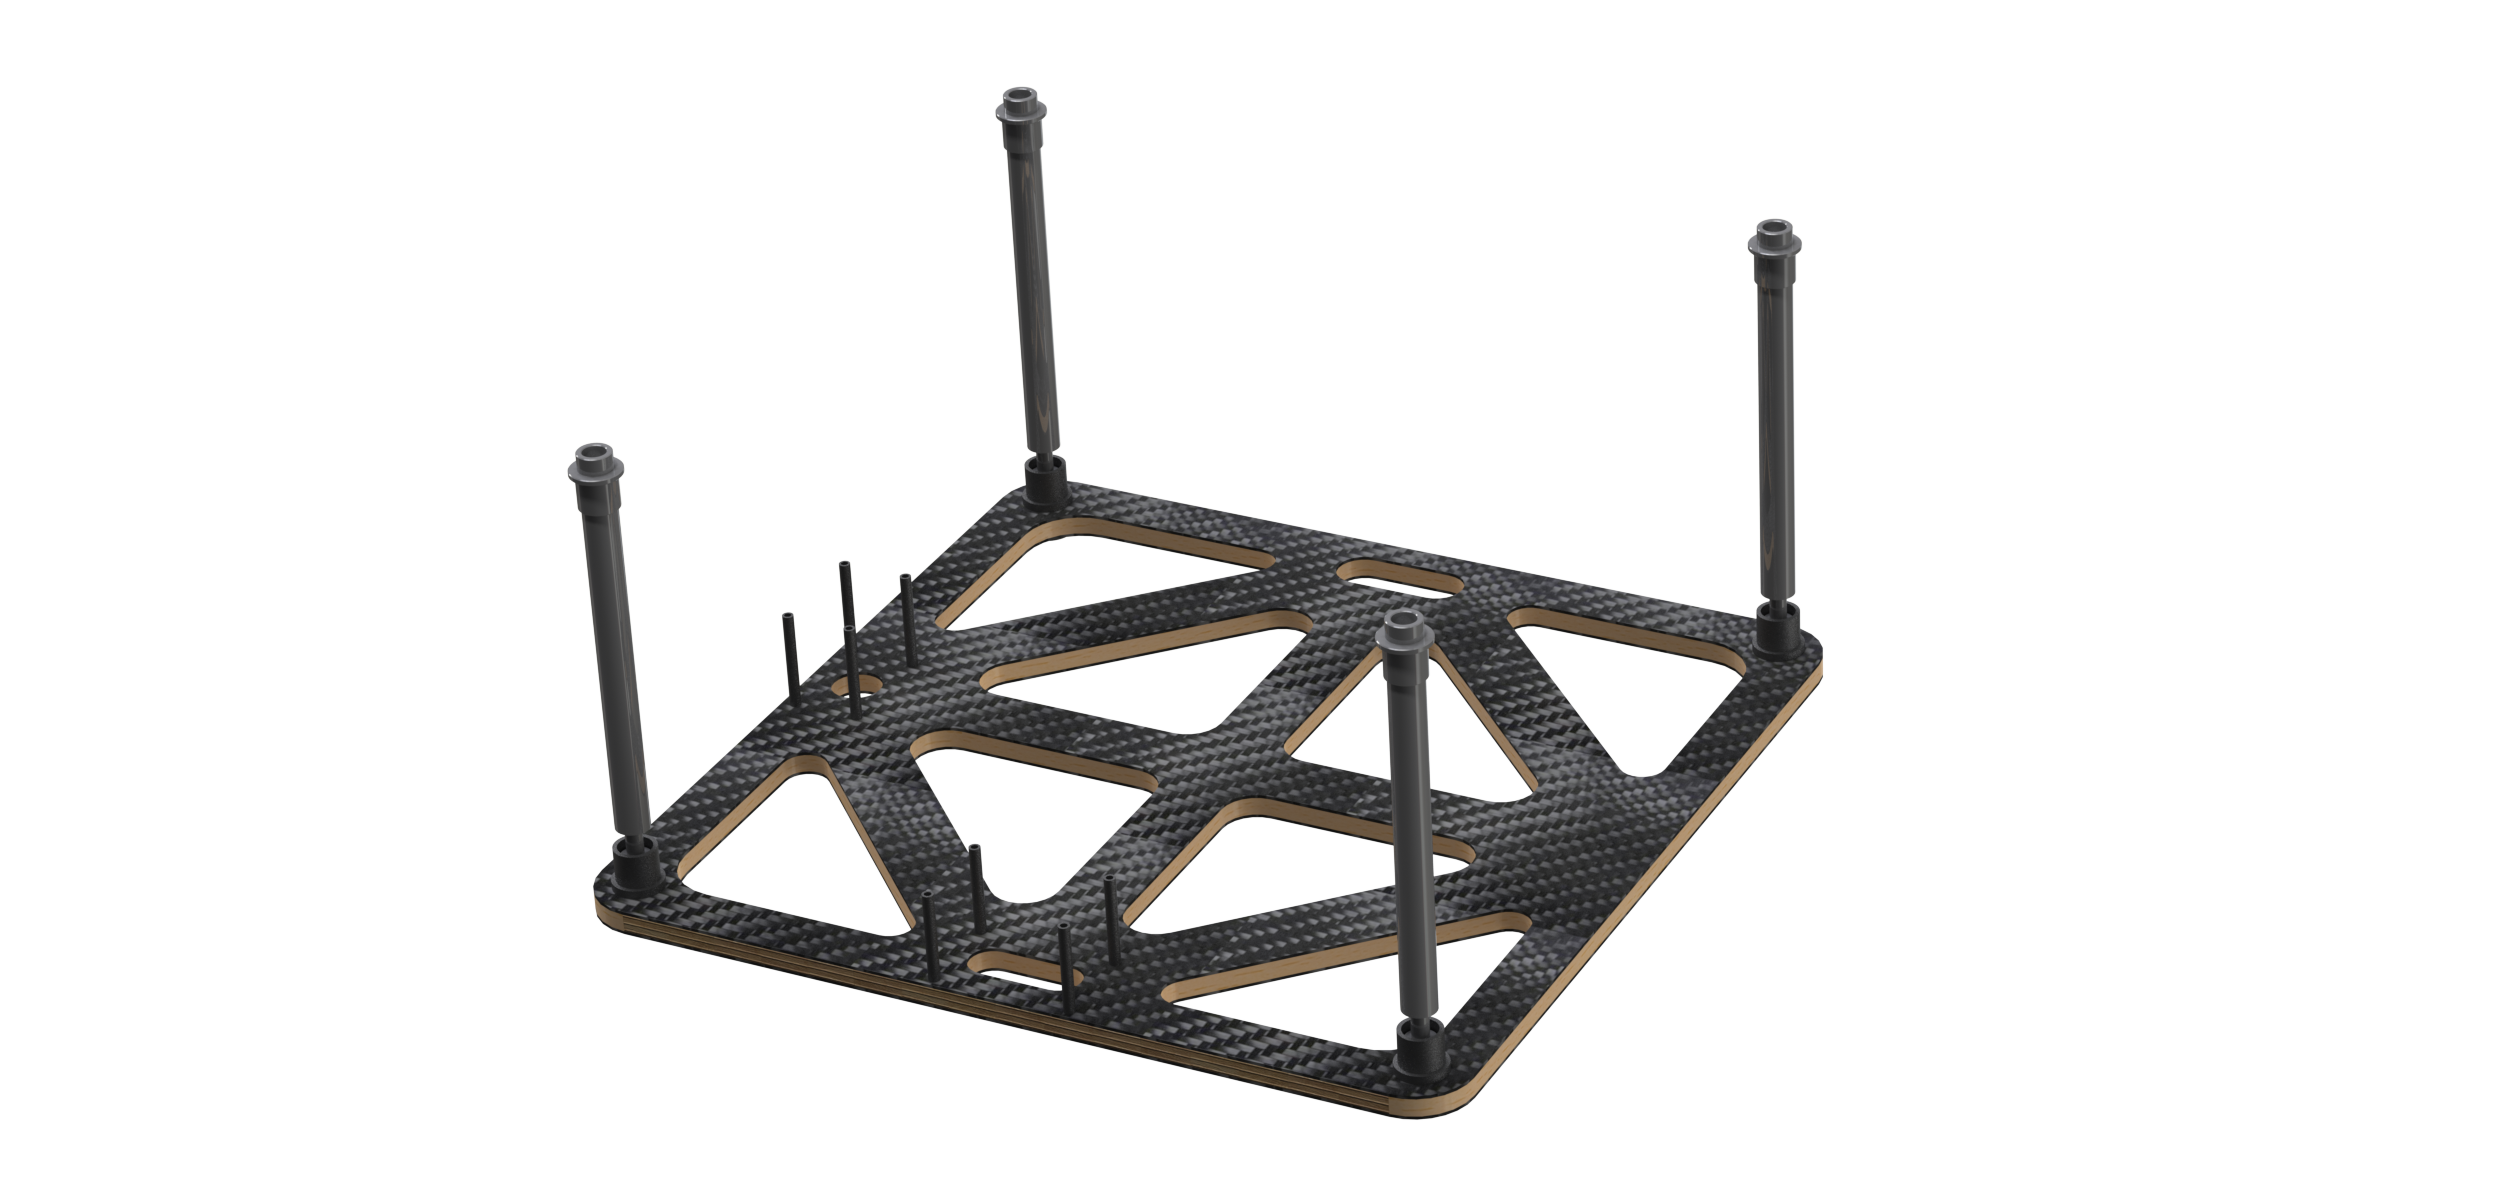
\includegraphics[width=0.6\textwidth]{render_belly.png}
	\vspace{-0.5cm}
	\caption{New landing gear for robot interaction.}
	\label{fig:payload-mech}
\end{figure}

\subsection*{Sensor suite} \label{subsec:payload-sensors}

\subsubsection*{GNC sensors}

The GNC sensor suite used for control is comprised of the Pixhawk’s inertial measurement unit (accelerometer, gyroscope, barometer, and compass), a PX4Flow optical flow camera, an external compass, and a LIDAR-Lite laser altitude sensor. The PX4 flight stack running on the Pixhawk is responsible to fuse all of this data, as explained in the \textit{Control System Architecture} section. 

\subsubsection*{Mission sensors}

The mission sensors include the four Intel RealSense 3D camera used for robot and obstacle detection and the Point Grey Firefly camera for visual localization. Their use is described in the \textit{Guidance, Navigation, and Control} section.

We have also integrated switches under the landing gear surface. With one switch under each landing leg, we can detect when legs touch the ground individually. This feedback is useful for autonomous landings or takeoffs. With another switch in the middle of the landing gear surface, we can detect physical interactions with ground robots. These switches are connected to an Arduino Nano, which is connected to the onboard computer through USB. The switch states are relayed to the computer through ROS messages with a \texttt{rosserial\_arduino} node and are then processed by the decision-making module.

\subsection*{Communications} \label{subsec:payload-comm}

Robot Operating System (ROS) is used to coordinate software communication between sensors, data processing, and decision-making modules. With its architecture, ROS allows for decentralized computation, which makes offboard processing possible through a Wi-Fi connection. However, offboard processing of the sensor data requires a high-bandwidth connection, but the wireless bands are cluttered by the teams running their own network. Therefore, during the IARC performance, the offboard computer is only used for monitoring through a 5~GHz network.

An RC receiver and a transmitter is used to activate offboard mode or for manual control when testing. A second RC receiver is used for the kill switch transmitter.

\subsection*{Power management system} \label{subsec:payload-power}

Our system is powered by two battery packs containing 4 lithium-ion polymer cells each. The three main systems of our vehicle are powered this way, that is the propulsion system, the flight controller and sensors system, and the onboard computer. The propulsion system is powered through the kill switch, as mentioned before. The Pixhawk is powered by a 5~V regulator (LM2678 from Texas Instruments). The onboard computer is powered through a 12~V DC power regulator (Murata UWE-12/10-Q12P-C).
